% ================================================================
% The Retrieve and Connect version of latex/starters/targeted/KS3/circles/circlesIntroductoryStarters_workedSolutions.tex
%
% This is the same deck as the one above, made by renaming the titles in it.
% Every slide that was a numbered starter is now titled
% "Retrieve and Connect", and the word is renamed wherever else a title
% used it. Nothing outside a title has been changed.
%
%   made from           latex/starters/targeted/KS3/circles/circlesIntroductoryStarters_workedSolutions.tex
%   retitling rules     version 1
%
% Please don't edit this file. It is written again from the one it was
% made from whenever that changes, so an edit here would be lost - edit
% that file instead and this one follows.
% ================================================================
% Root file used ashow macros
\documentclass{beamer}
\usepackage{tikz}
\usetikzlibrary{calc,arrows.meta,patterns}
\usepackage{xcolor}
\usepackage{multicol}
\usepackage{amsmath}

% ================================================================
% Answer-overlay helpers
% ================================================================
\newcommand{\ablank}[1]{%
  \alt<2>{\textcolor{red}{#1}}{\underline{\phantom{#1}}}%
}
\newcommand{\ashow}[1]{\uncover<2->{\textcolor{red}{\small #1}}}
\newcommand{\ashowq}[1]{\alt<2->{\textcolor{red}{\small #1}}{?}}

% Answers drawn straight on to a TikZ diagram, revealed on overlay 2 like \ashow.
% Space is reserved on overlay 1, so the diagram does not move between slides.
\usetikzlibrary{overlay-beamer-styles}
\tikzset{
  ans/.style     = {red, thick, visible on=<2->},
  ansfill/.style = {red!15, visible on=<2->},
  anslab/.style  = {red, font=\tiny, visible on=<2->},
}

\title{Circles: Parts, Perimeter \& Pi}
\author{}
\date{}

\begin{document}

\frame{\titlepage}

%------------------------------------------------
% CONTENTS
%------------------------------------------------
\begin{frame}{Contents}
\small
\begin{columns}[T]
\column{0.5\textwidth}
\textbf{Questions and short answers}
\begin{itemize}
  \item \hyperlink{q-st1}{\beamergotobutton{Retrieve and Connect 1}}
  \item \hyperlink{q-st2}{\beamergotobutton{Retrieve and Connect 2}}
  \item \hyperlink{q-st3}{\beamergotobutton{Retrieve and Connect 3}}
  \item \hyperlink{q-st4}{\beamergotobutton{Retrieve and Connect 4}}
\end{itemize}
\column{0.5\textwidth}
\textbf{Worked solutions}
\begin{itemize}
  \item \hyperlink{work-st1}{\beamergotobutton{Retrieve and Connect 1}}
  \item \hyperlink{work-st2}{\beamergotobutton{Retrieve and Connect 2}}
  \item \hyperlink{work-st3}{\beamergotobutton{Retrieve and Connect 3}}
  \item \hyperlink{work-st4}{\beamergotobutton{Retrieve and Connect 4}}
\end{itemize}
\end{columns}
\end{frame}

%------------------------------------------------
% SLIDE 1: Arithmetic, Lengths & Decimals (No Circles)
%------------------------------------------------
\begin{frame}{Retrieve and Connect}
\hypertarget{q-st1}{}

\begin{columns}

\column{0.3\textwidth}
\begin{center}
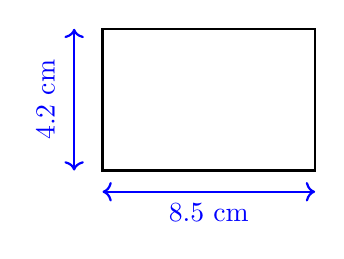
\begin{tikzpicture}[scale=0.9]
  % Rectangle for perimeter
  \draw[thick] (0,0) rectangle (3,2);
  \draw[blue, thick, <->] (0,-0.3) -- (3,-0.3);
  \node[blue] at (1.5,-0.6) {$8.5$ cm};
  \draw[blue, thick, <->] (-0.4,0) -- (-0.4,2);
  \node[blue, rotate=90] at (-0.8,1) {$4.2$ cm};
  
\end{tikzpicture}
\end{center}

\column{0.7\textwidth}
\small
\begin{enumerate}
    \begin{multicols}{2}
        \item $13 + 9 = \ashowq{22}$
        \item $5.8 - 1.9 = \ashowq{3.9}$
    \end{multicols}
    \begin{multicols}{2}
        \item $6 \times 8 = \ashowq{48}$
        \item $4 \times 3.5 \ \ashowq{14}$
  \end{multicols}
  \item Round $3.14159$ to 2 decimal places. \ashow{3.14}
  \item A pencil is $12.8$ cm long. How many millimetres is this? \ablank{128 mm}
\end{enumerate}

\begin{enumerate}
  \setcounter{enumi}{4}
  \item Find the perimeter of the rectangle shown. \ashow{25.4 cm}
  \item The perimeter of a square is $26$ cm. What is the length of one side? \ashow{6.5 cm}
  \item  The perimeter of an equilateral triangle is $12.9$ cm. 
    Find the length of one side, and then the perimeter of a regular hexagon with the same side length. \ashow{$4.3$ cm; hexagon: $25.8$ cm}
\end{enumerate}

\end{columns}
\end{frame}

%------------------------------------------------
% Starter 1 Worked Solutions
%------------------------------------------------
\begin{frame}{Worked Solution: Retrieve and Connect 1, Question 1}
\hypertarget{work-st1}{}
\small
\textbf{Question:} \(13+9\).

\textbf{Worked Solution:} Use \(9=10-1\):
\(13+9=13+10-1=23-1=\ablank{22}\).
\end{frame}

\begin{frame}{Worked Solution: Retrieve and Connect 1, Question 2}
\small
\textbf{Question:} \(5.8-1.9\).

\textbf{Worked Solution:} Subtract \(2\) and add back \(0.1\):
\(5.8-1.9=5.8-2+0.1=3.8+0.1=\ablank{3.9}\).
\end{frame}

\begin{frame}{Worked Solution: Retrieve and Connect 1, Question 3}
\small
\textbf{Question:} \(6\times8\).

\textbf{Worked Solution:} Six groups of eight:
\(6\times8=\ablank{48}\).
\end{frame}

\begin{frame}{Worked Solution: Retrieve and Connect 1, Question 4}
\small
\textbf{Question:} \(4\times3.5\).

\textbf{Worked Solution:} Split \(3.5=3+0.5\):
\(4\times3.5=4\times3+4\times0.5=12+2=\ablank{14}\).
\end{frame}

\begin{frame}{Worked Solution: Retrieve and Connect 1, Question 5}
\small
\textbf{Question:} Round \(3.14159\) to 2 decimal places.

\textbf{Worked Solution:} The second decimal digit is \(4\), and the next digit is \(1<5\), so leave the \(4\) unchanged:
\(3.14159\approx\ablank{3.14}\).
\end{frame}

\begin{frame}{Worked Solution: Retrieve and Connect 1, Question 6}
\small
\textbf{Question:} A pencil is \(12.8\) cm long. How many millimetres is this?

\textbf{Worked Solution:} Since \(1\text{ cm}=10\text{ mm}\),
\(12.8\text{ cm}=12.8\times10=\ablank{128\text{ mm}}\).
\end{frame}

\begin{frame}{Worked Solution: Retrieve and Connect 1, Question 7}
\small
\textbf{Question:} Find the perimeter of the rectangle shown.

\begin{center}
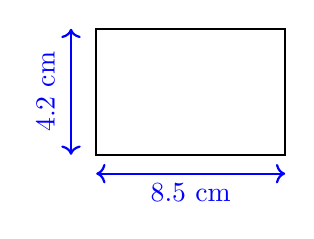
\begin{tikzpicture}[scale=0.8]
  \draw[thick] (0,0) rectangle (3,2);
  \draw[blue, thick, <->] (0,-0.3) -- (3,-0.3);
  \node[blue] at (1.5,-0.6) {$8.5$ cm};
  \draw[blue, thick, <->] (-0.4,0) -- (-0.4,2);
  \node[blue, rotate=90] at (-0.8,1) {$4.2$ cm};
\end{tikzpicture}
\end{center}

\textbf{Worked Solution:} Perimeter \(=2(\text{length}+\text{width})=2(8.5+4.2)=2(12.7)=\ablank{25.4\text{ cm}}\).
\end{frame}

\begin{frame}{Worked Solution: Retrieve and Connect 1, Question 8}
\small
\textbf{Question:} The perimeter of a square is \(26\) cm. What is the length of one side?

\textbf{Worked Solution:} A square has \(4\) equal sides, so
\(s=\frac{26}{4}=\ablank{6.5\text{ cm}}\).
\end{frame}

\begin{frame}{Worked Solution: Retrieve and Connect 1, Question 9}
\small
\textbf{Question:} The perimeter of an equilateral triangle is \(12.9\) cm. Find the length of one side, and then the perimeter of a regular hexagon with the same side length.

\textbf{Worked Solution:} An equilateral triangle has \(3\) equal sides:
\(s=\frac{12.9}{3}=\ablank{4.3\text{ cm}}\).

A regular hexagon has \(6\) equal sides:
\(P=6\times4.3=\ablank{25.8\text{ cm}}\).
\end{frame}

%------------------------------------------------
% SLIDE 2: Arithmetic + Radius, Diameter, Chord
%------------------------------------------------
\begin{frame}{Retrieve and Connect}
\hypertarget{q-st2}{}
\vspace{-2em}
\begin{columns}

\column{0.3\textwidth}
\begin{center}
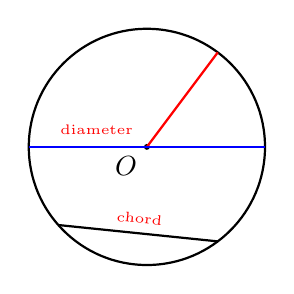
\begin{tikzpicture}[scale=0.75]
  % Circle
  \draw[thick] (0,0) circle (2cm);

  % Center
  \fill (0,0) circle (0.05);
  \node[below left] at (0,0) {$O$};

  % Radius
  \draw[red, thick] (0,0) -- (1.2,1.6);

  % Diameter
  \draw[blue, thick] (-2,0) -- (2,0);

  % Chord (not through center)
  \draw[thick] (-1.5,-1.323) -- (1.2,-1.6);

  % --- Q5 answer: name the lines on the diagram ---
  \node[anslab, above] at (-0.85,0.05) {diameter};
  \node[anslab, above, rotate=-6] at (-0.15,-1.46) {chord};
\end{tikzpicture}
\end{center}

\column{0.7\textwidth}
\small
\begin{enumerate}
\begin{multicols}{2}
  \item $24 \div 6$ \ashow{$=4$}
  \item $72 \div 8$ \ashow{$=9$}
  \end{multicols}
  \begin{multicols}{2}
  \item Double $15.5$ \ashow{$=31$}
  \item Halve $31.4$ \ashow{$=15.7$}
  \end{multicols}
  \item How many centimetres in $1.2$ metres? \ashow{120 cm}
  \item True or false? $2.5 \times 4 = 10$ \ashow{True}
\end{enumerate}

\begin{enumerate}
  \setcounter{enumi}{4}
  \item On the diagram, which line is the \textbf{diameter}? 
    How is it different from a chord? \ashow{A diameter passes through the centre.}
  \item If the radius of a circle is $7$ cm, what is its diameter? \ashow{14 cm}
  \item The diameter of a circle is $18$ mm. Find its radius. \ablank{9 mm}
  \item A chord of length $8$ cm is drawn inside a circle of radius $5$ cm.
    Is the chord a diameter? Why, or why not?. \ashow{No; a diameter would be $10$ cm.}
\end{enumerate}

\end{columns}
\end{frame}

%------------------------------------------------
% Starter 2 Worked Solutions
%------------------------------------------------
\begin{frame}{Worked Solution: Retrieve and Connect 2, Question 1}
\hypertarget{work-st2}{}
\small
\textbf{Question:} \(24\div6\).

\textbf{Worked Solution:} Since \(6\times4=24\), \(24\div6=\ablank{4}\).
\end{frame}

\begin{frame}{Worked Solution: Retrieve and Connect 2, Question 2}
\small
\textbf{Question:} \(72\div8\).

\textbf{Worked Solution:} Since \(8\times9=72\), \(72\div8=\ablank{9}\).
\end{frame}

\begin{frame}{Worked Solution: Retrieve and Connect 2, Question 3}
\small
\textbf{Question:} Double \(15.5\).

\textbf{Worked Solution:} \(2\times15.5=15.5+15.5=\ablank{31}\).
\end{frame}

\begin{frame}{Worked Solution: Retrieve and Connect 2, Question 4}
\small
\textbf{Question:} Halve \(31.4\).

\textbf{Worked Solution:} \(31.4\div2=\ablank{15.7}\).
\end{frame}

\begin{frame}{Worked Solution: Retrieve and Connect 2, Question 5}
\small
\textbf{Question:} How many centimetres in \(1.2\) metres?

\textbf{Worked Solution:} \(1\text{ m}=100\text{ cm}\), so
\(1.2\text{ m}=1.2\times100=\ablank{120\text{ cm}}\).
\end{frame}

\begin{frame}{Worked Solution: Retrieve and Connect 2, Question 6}
\small
\textbf{Question:} True or false? \(2.5\times4=10\).

\textbf{Worked Solution:} \(2.5\times4=10\), so the statement is \ablank{True}.
\end{frame}

\begin{frame}{Worked Solution: Retrieve and Connect 2, Question 7}
\small
\textbf{Question:} On the diagram, which line is the \textbf{diameter}? How is it different from a chord?

\begin{center}
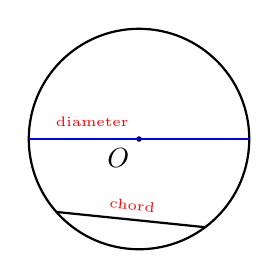
\begin{tikzpicture}[scale=0.7]
  \draw[thick] (0,0) circle (2cm);
  \fill (0,0) circle (0.05);
  \node[below left] at (0,0) {$O$};
  \draw[blue, thick] (-2,0) -- (2,0);
  \draw[thick] (-1.5,-1.323) -- (1.2,-1.6);
  \node[anslab, above] at (-0.85,0.05) {diameter};
  \node[anslab, above, rotate=-6] at (-0.15,-1.46) {chord};
\end{tikzpicture}
\end{center}

\textbf{Worked Solution:} The blue line is \ashow{the diameter}. A diameter is a chord that \ashow{passes through the centre}.
\end{frame}

\begin{frame}{Worked Solution: Retrieve and Connect 2, Question 8}
\small
\textbf{Question:} If the radius of a circle is \(7\) cm, what is its diameter?

\textbf{Worked Solution:} Diameter \(d=2r=2(7)=\ablank{14\text{ cm}}\).
\end{frame}

\begin{frame}{Worked Solution: Retrieve and Connect 2, Question 9}
\small
\textbf{Question:} The diameter of a circle is \(18\) mm. Find its radius.

\textbf{Worked Solution:} Radius \(r=\frac{d}{2}=\frac{18}{2}=\ablank{9\text{ mm}}\).
\end{frame}

\begin{frame}{Worked Solution: Retrieve and Connect 2, Question 10}
\small
\textbf{Question:} A chord of length \(8\) cm is drawn inside a circle of radius \(5\) cm. Is the chord a diameter? Why, or why not?

\textbf{Worked Solution:} A diameter would have length \(2r=2(5)=\ablank{10\text{ cm}}\). Since the chord is only \(8\) cm, \ashow{it is not a diameter; a diameter would be \(10\) cm.}
\end{frame}

%------------------------------------------------
% SLIDE 3: Arithmetic + Segments, Sectors, Arcs, Tangents
%------------------------------------------------
\begin{frame}{Retrieve and Connect}
\hypertarget{q-st3}{}
\vspace{-2em}

\begin{columns}

\column{0.35\textwidth}

\begin{center}
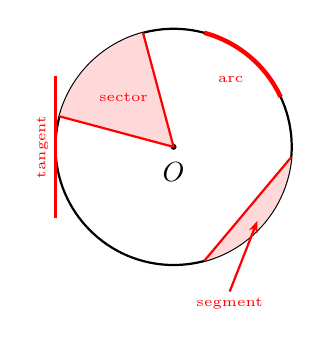
\begin{tikzpicture}[scale=0.75]
  % Circle
  \draw[thick] (0,0) circle (2cm);
  \fill (0,0) circle (0.05);
  \node[below] at (0,-0.1) {$O$};

  % --- Q6 answers: drawn on the circle ---
  % Sector
  \fill[ansfill] (0,0) -- (105:2) arc (105:165:2) -- cycle;
  \draw[ans] (0,0) -- (105:2);
  \draw[ans] (0,0) -- (165:2);
  \node[anslab] at (135:1.2) {sector};

  % Arc
  \draw[ans, ultra thick] (25:2) arc (25:75:2);
  \node[anslab] at (50:1.5) {arc};

  % Tangent
  \draw[ans] (-2,-1.2) -- (-2,1.2);
  \node[anslab, rotate=90] at (-2.22,0) {tangent};

  % Segment
  \fill[ansfill] (-75:2) arc (-75:-5:2) -- cycle;
  \draw[ans] (-75:2) -- (-5:2);
  \draw[ans, -{Stealth[length=1.5mm]}] (0.95,-2.45) -- (1.42,-1.25);
  \node[anslab] at (0.95,-2.65) {segment};
\end{tikzpicture}

\vspace{3em}

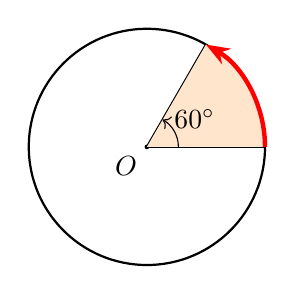
\begin{tikzpicture}[scale=1]
  % Circle
  \draw[thick] (0,0) circle (1.5cm);
  
  % Centre
  \fill (0,0) circle (0.03);
  \node[below left] at (0,0) {$O$};
  
  % Radii that bound the 60° sector
  \draw[thick] (0,0) -- (0:1.5);          % right horizontal radius
  \draw[thick] (0,0) -- (60:1.5);         % radius at 60°
  
  % Optional: shade the sector lightly
  \fill[orange!20] (0,0) -- (0:1.5) arc (0:60:1.5) -- cycle;

  % Highlight the arc (thick, coloured, with arrow)
  \draw[red, ultra thick, -{Stealth[length=3mm]}] 
    (0:1.5) arc (0:60:1.5);
  
  % Angle arc and label
  \draw[->] (0.4,0) arc (0:60:0.4);
  \node at (30:0.7) {$60^\circ$};
  
\end{tikzpicture}

\end{center}

\column{0.65\textwidth}
\small
\begin{enumerate}
\begin{multicols}{2}
  \item $3.2 \times 5$ \ashow{$=16$}
  \item $1.8 \times 4$ \ashow{$=7.2$}
  \end{multicols}
  \begin{multicols}{2}
    \item  $45 \div 10$ \ashow{$=4.5$}
    \item $90 \div 100$ \ashow{$=0.9$}
  \end{multicols}
  \item What is $\frac{1}{4}$ of $360^\circ$? \ashow{$90^\circ$}
\end{enumerate}

\begin{enumerate}
  \setcounter{enumi}{5}
  \item Copy the diagram, and draw with labels:
    \begin{multicols}{2}
    \begin{itemize}
      \item A sector
      \item An arc
      \item A tangent
      \item A segment
    \end{itemize}
    \end{multicols}
  \item If the radius is $6$ cm, what is the whole circumference? (Use $\pi \approx 3.14$) \ashow{$37.68$ cm}
  \item For the sector shown, what fraction of the circumference is the arc length? Calculate the arc length if the whole circle has a circumference of 24cm. \ashow{$\frac{1}{6}$; $4$ cm}

\end{enumerate}

\end{columns}
\end{frame}

%------------------------------------------------
% Starter 3 Worked Solutions
%------------------------------------------------
\begin{frame}{Worked Solution: Retrieve and Connect 3, Question 1}
\hypertarget{work-st3}{}
\small
\textbf{Question:} \(3.2\times5\).

\textbf{Worked Solution:} Split \(3.2=3+0.2\):
\(3.2\times5=3\times5+0.2\times5=15+1=\ablank{16}\).
\end{frame}

\begin{frame}{Worked Solution: Retrieve and Connect 3, Question 2}
\small
\textbf{Question:} \(1.8\times4\).

\textbf{Worked Solution:} \(1.8\times4=1\times4+0.8\times4=4+3.2=\ablank{7.2}\).
\end{frame}

\begin{frame}{Worked Solution: Retrieve and Connect 3, Question 3}
\small
\textbf{Question:} \(45\div10\).

\textbf{Worked Solution:} Dividing by \(10\) moves the digits one place to the right:
\(45\div10=\ablank{4.5}\).
\end{frame}

\begin{frame}{Worked Solution: Retrieve and Connect 3, Question 4}
\small
\textbf{Question:} \(90\div100\).

\textbf{Worked Solution:} Dividing by \(100\) moves the digits two places to the right:
\(90\div100=\ablank{0.9}\).
\end{frame}

\begin{frame}{Worked Solution: Retrieve and Connect 3, Question 5}
\small
\textbf{Question:} What is \(\frac14\) of \(360^\circ\)?

\textbf{Worked Solution:} \(\frac14\times360^\circ=\frac{360^\circ}{4}=\ablank{90^\circ}\).
\end{frame}

\begin{frame}{Worked Solution: Retrieve and Connect 3, Question 6}
\small
\textbf{Question:} Copy the diagram, and draw with labels: a sector, an arc, a tangent, and a segment.

\textbf{Worked Solution:} The labelled parts are shown below.

\begin{center}
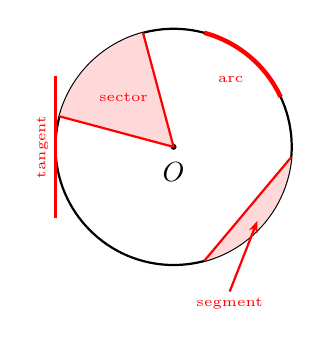
\begin{tikzpicture}[scale=0.75]
  \draw[thick] (0,0) circle (2cm);
  \fill (0,0) circle (0.05);
  \node[below] at (0,-0.1) {$O$};

  % Sector
  \fill[ansfill] (0,0) -- (105:2) arc (105:165:2) -- cycle;
  \draw[ans] (0,0) -- (105:2);
  \draw[ans] (0,0) -- (165:2);
  \node[anslab] at (135:1.2) {sector};

  % Arc
  \draw[ans, ultra thick] (25:2) arc (25:75:2);
  \node[anslab] at (50:1.5) {arc};

  % Tangent
  \draw[ans] (-2,-1.2) -- (-2,1.2);
  \node[anslab, rotate=90] at (-2.22,0) {tangent};

  % Segment
  \fill[ansfill] (-75:2) arc (-75:-5:2) -- cycle;
  \draw[ans] (-75:2) -- (-5:2);
  \draw[ans, -{Stealth[length=1.5mm]}] (0.95,-2.45) -- (1.42,-1.25);
  \node[anslab] at (0.95,-2.65) {segment};
\end{tikzpicture}
\end{center}
\end{frame}

\begin{frame}{Worked Solution: Retrieve and Connect 3, Question 7}
\small
\textbf{Question:} If the radius is \(6\) cm, what is the whole circumference? Use \(\pi\approx3.14\).

\textbf{Worked Solution:} \(C=2\pi r\approx2(3.14)(6)=\ablank{37.68\text{ cm}}\).
\end{frame}

\begin{frame}{Worked Solution: Retrieve and Connect 3, Question 8}
\small
\textbf{Question:} For the sector shown, what fraction of the circumference is the arc length? Calculate the arc length if the whole circle has a circumference of \(24\) cm.

\textbf{Worked Solution:} The sector angle is \(60^\circ\), so the fraction is
\(\frac{60}{360}=\ablank{\frac16}\).

The arc length is therefore
\(\frac16\times24=\ablank{4\text{ cm}}\).
\end{frame}

%------------------------------------------------
% SLIDE 4: Arithmetic + Labelling, Pi, Diameter
%------------------------------------------------
\begin{frame}{Retrieve and Connect}
\hypertarget{q-st4}{}
\vspace{-2em}

\begin{columns}

\column{0.3\textwidth}
\begin{center}
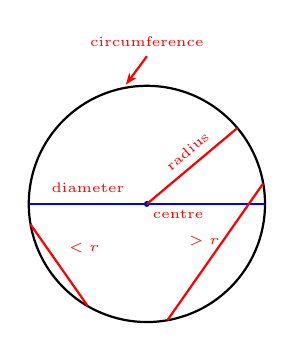
\begin{tikzpicture}[scale=0.75]
  % Circle with labels
  \draw[thick] (0,0) circle (2cm);
  \fill (0,0) circle (0.05);

  \draw[blue, thick] (-2,0) -- (2,0);

  \draw[red, thick] (0,0) -- (40:2);

  % --- Q8 answer: label the parts on the diagram ---
  \node[anslab, below right, inner sep=2pt] at (0,0) {centre};
  \node[anslab, above, rotate=40] at (40:1.1) {radius};
  \node[anslab, above] at (-1,0.02) {diameter};
  \draw[ans, -{Stealth[length=1.5mm]}] (0,2.5) -- (100:2.05);
  \node[anslab, above] at (0,2.5) {circumference};

  % --- Q9 answer: a chord shorter than the radius ---
  \draw[ans] (190:2) -- (240:2);
  \node[anslab] at (215:1.3) {$<r$};

  % --- Q10 answer: a chord longer than the radius ---
  \draw[ans] (-80:2) -- (10:2);
  \node[anslab] at (-33:1.15) {$>r$};
\end{tikzpicture}

\end{center}

\column{0.7\textwidth}
\small
\begin{enumerate}
\begin{multicols}{2}
  \item $12 \times 3 $ \ashow{$=36$}
  \item $4 \times 3.14$ \ashow{$=12.56$}
\end{multicols}
\begin{multicols}{2}
  \item $6.28 \div 2 $ \ashow{$=3.14$} 
  \item $ 9.42 \div 3$ \ashow{$=3.14$}
  \end{multicols}
  \item Round $3.14159265$ to 3 decimal places. \ashow{3.142}
  \begin{multicols}{2}
  \item Double $3.14$ \ashow{$=6.28$}
  \item halve $12.56$ \ashow{$=6.28$}
  \end{multicols}
\end{enumerate}
\vspace{-0.5em}
\begin{enumerate}
  \setcounter{enumi}{7}
  \item Copy and label on the diagram: 
    centre, radius, diameter, circumference.
    \item Draw a chord on the diagram shorter than the radius
    \item Draw a chord on the diagram longer than the radius
  
  \item If the diameter is $8$ cm, what is:
    \begin{itemize}
      \item the radius? \ashow{$4$ cm}
      \item the circumference? ($\pi \approx 3.14$) \ashow{$25.12$ cm}
    \end{itemize}
 
\end{enumerate}

\end{columns}
\end{frame}

%------------------------------------------------
% Starter 4 Worked Solutions
%------------------------------------------------
\begin{frame}{Worked Solution: Retrieve and Connect 4, Question 1}
\hypertarget{work-st4}{}
\small
\textbf{Question:} \(12\times3\).

\textbf{Worked Solution:} \(12\times3=10\times3+2\times3=30+6=\ablank{36}\).
\end{frame}

\begin{frame}{Worked Solution: Retrieve and Connect 4, Question 2}
\small
\textbf{Question:} \(4\times3.14\).

\textbf{Worked Solution:} \(4\times3.14=4\times3+4\times0.14=12+0.56=\ablank{12.56}\).
\end{frame}

\begin{frame}{Worked Solution: Retrieve and Connect 4, Question 3}
\small
\textbf{Question:} \(6.28\div2\).

\textbf{Worked Solution:} Half of \(6.28\) is \(3.14\), so \(6.28\div2=\ablank{3.14}\).
\end{frame}

\begin{frame}{Worked Solution: Retrieve and Connect 4, Question 4}
\small
\textbf{Question:} \(9.42\div3\).

\textbf{Worked Solution:} Since \(3\times3.14=9.42\), \(9.42\div3=\ablank{3.14}\).
\end{frame}

\begin{frame}{Worked Solution: Retrieve and Connect 4, Question 5}
\small
\textbf{Question:} Round \(3.14159265\) to 3 decimal places.

\textbf{Worked Solution:} The third decimal digit is \(1\), and the next digit is \(5\), so round up:
\(3.14159265\approx\ablank{3.142}\).
\end{frame}

\begin{frame}{Worked Solution: Retrieve and Connect 4, Question 6}
\small
\textbf{Question:} Double \(3.14\).

\textbf{Worked Solution:} \(2\times3.14=\ablank{6.28}\).
\end{frame}

\begin{frame}{Worked Solution: Retrieve and Connect 4, Question 7}
\small
\textbf{Question:} Halve \(12.56\).

\textbf{Worked Solution:} \(12.56\div2=\ablank{6.28}\).
\end{frame}

\begin{frame}{Worked Solution: Retrieve and Connect 4, Question 8}
\small
\textbf{Question:} Copy and label on the diagram: centre, radius, diameter, circumference.

\begin{center}
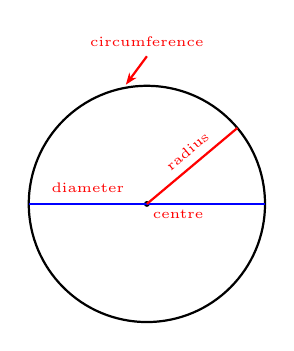
\begin{tikzpicture}[scale=0.75]
  \draw[thick] (0,0) circle (2cm);
  \fill (0,0) circle (0.05);
  \draw[blue, thick] (-2,0) -- (2,0);
  \draw[red, thick] (0,0) -- (40:2);

  \node[anslab, below right, inner sep=2pt] at (0,0) {centre};
  \node[anslab, above, rotate=40] at (40:1.1) {radius};
  \node[anslab, above] at (-1,0.02) {diameter};
  \draw[ans, -{Stealth[length=1.5mm]}] (0,2.5) -- (100:2.05);
  \node[anslab, above] at (0,2.5) {circumference};
\end{tikzpicture}
\end{center}

\textbf{Worked Solution:} The labels are shown in red. The centre is \(O\), the radius is half the diameter, the diameter passes through the centre, and the circumference is the distance around the circle.
\end{frame}

\begin{frame}{Worked Solution: Retrieve and Connect 4, Question 9}
\small
\textbf{Question:} Draw a chord on the diagram shorter than the radius.

\begin{center}
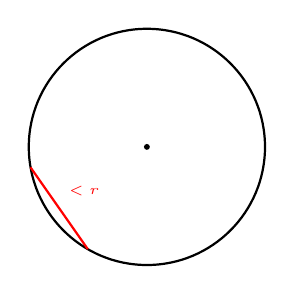
\begin{tikzpicture}[scale=0.75]
  \draw[thick] (0,0) circle (2cm);
  \fill (0,0) circle (0.05);

  \draw[ans] (190:2) -- (240:2);
  \node[anslab] at (215:1.3) {$<r$};
\end{tikzpicture}
\end{center}

\textbf{Worked Solution:} One possible chord is drawn below; it is labelled \(<r\).
\end{frame}

\begin{frame}{Worked Solution: Retrieve and Connect 4, Question 10}
\small
\textbf{Question:} Draw a chord on the diagram longer than the radius.

\begin{center}
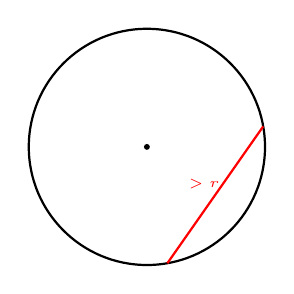
\begin{tikzpicture}[scale=0.75]
  \draw[thick] (0,0) circle (2cm);
  \fill (0,0) circle (0.05);

  \draw[ans] (-80:2) -- (10:2);
  \node[anslab] at (-33:1.15) {$>r$};
\end{tikzpicture}
\end{center}

\textbf{Worked Solution:} One possible chord is drawn below; it is labelled \(>r\).
\end{frame}

\begin{frame}{Worked Solution: Retrieve and Connect 4, Question 11}
\small
\textbf{Question:} If the diameter is \(8\) cm, what is the radius and the circumference? Use \(\pi\approx3.14\).

\textbf{Worked Solution:} Radius \(r=\frac{8}{2}=\ablank{4\text{ cm}}\).

Circumference \(C=\pi d\approx3.14\times8=\ablank{25.12\text{ cm}}\).
\end{frame}

\end{document}